\documentclass[11pt]{article}
\usepackage{graphicx}
\newcommand{\ndata}{{N_{\rm data}}}
\newcommand{\ydata}{{y_{\rm data}}}
\newcommand{\xdata}{{x_{\rm data}}}
\newcommand{\nparam}{{N_{\rm param}}}
\newcommand{\nnuis}{{N_{\rm nuis}}}
\newcommand{\neff}{{N_{\rm eff}}}
\newcommand{\chisq}{{\chi^{2}}}
\author{Surhud More}
\title{Degrees of freedom counting and $\chisq$}
\begin{document}
\maketitle

This document tries to illustrate how degrees of freedom should be counted in
the cosmic shear analyses. Of course, it may not matter much to the final
results, but it is such a basic thing, so it is better if we can get it right.

Let $\ndata$ be the number of data points in any measurement, $\nparam$
be the truly free parameters, $\nnuis$ be the number of prior constraints
that we use while fitting the data. There are two different ways we are
debating to compute the $\chisq$ and the degrees of freedom and we want to
understand which way makes more sense and in which limit.

The first way (what we are currently doing in the cosmic shear paper) is to
compute the $\chisq$ only from the likelihood. This method ignores the priors
completely while quoting the $\chisq$, let us call this $\chisq_{\rm lik}$.
Then he counts the degrees of freedom as $\ndata-\nparam-\nnuis$.

The second way (what I am proposing) is to compute the $\chisq$ from the
posterior itself, that is by adding the $\chisq$ contribution from the priors,
let us call it $\chisq_{\rm post}$.  In my case, I also calculate the degrees
of freedom as $(\ndata+\nnuis)-(\nparam+\nnuis)$.

We want to understand which of these ways is the correct way to do things and
in what limit.

Therefore I simulate data from a simple linear model $\ydata=a+b\times
\xdata+\epsilon$, where $\epsilon$ has some error distribution. Now I leave the
parameter $b$ completely free and add a Gaussian prior constraint on the
parameter $a$. I will use $\ndata=10$. 

According to the first way, the $\chisq_{\rm lik}$ should follow a $\chisq$
distribution with $\ndata-\nparam-\nnuis=\ndata-2$ degrees of freedom. On the
other hand, the second way predicts that $\chisq_{\rm post}$ should follow a
$\chisq$ distribution with $\ndata-1$ degrees of freedom.

I will show two useful edge cases to demonstrate the validity of each of the
above equations. First case is the data driven case, i.e., when the prior is
effectively useless. The data can constrain the parameter much much better than
the prior information on the parameter $a$. The second case is the opposite
prior-driven case, where the prior on the parameter completely dominates the
posterior. For the two cases, all I have done is increase the scale of the
Gaussian prior constraint.

I generate a large number of simulated data sets, fit them with the simple
linear model and compute the distribution of $\chisq_{\rm lik}$ and
$\chisq_{\rm post}$ at the location of the best fit. The data driven case is
shown first in Figure~\ref{fig1} while the prior-driven case is shown in
Figure~\ref{fig2}. The distribution of $\chisq_{\rm post}$ is shown in the left
hand panels as the blue histogram, while that of $\chisq_{\rm lik}$ is shown in
the right hand panel as a histogram with the same color. The different solid
lines show the analytical $\chisq$ distribution with different degrees of
freedom.

It can be seen that in the data driven case, the first and the second way both
match the respective $\chisq$ distributions that they are designed to match.
However, in the prior-driven case, the first way fails to match the
$\chisq_{\rm lik}$ distribution, whereas the second way works perfectly fine to
match the $\chisq_{\rm post}$ distribution.

The conclusion is that we should always be using the second way, unless you
want to actually work out what the actual difference in the posterior compared
to the prior is. The mathematics behind how to work this out is given in Raveri
and Hu 2018 (but it unnecessary if we use the second way all throughout). I
think it is likely that the Raveri and Hu estimator can also be generalized
quite trivially for this second way as well (it does not even involve actual
computation of the $\neff$ as required in Raveri and Hu 2018).

It is also important to note that for most of the nuisance parameters that we
consider in our cosmic shear analysis, the posterior for the nuisance
parameters is most of the time dominated by the priors, rather than the data
itself. Thus we are in the second case, where the first way is not the correct
approach.

There are other reasons why the second way is also more appropriate. For
example, in the first way, any fixed parameters can be assumed to have delta
function priors, and will have to be subtracted off via $\nnuis$. This can
arbitrarily reduce the degrees of freedom. In the second way, these fixed
parameters never matter in either the calculation of $\chisq_{\rm post}$ or the
degrees of freedom.

\begin{figure*}
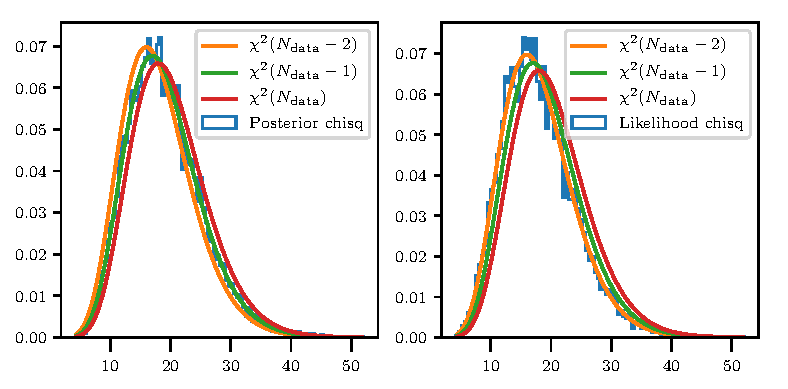
\includegraphics[scale=0.9]{Data_driven.pdf}
\caption{Data driven case: In this case, the first way of computing degrees of
freedom reproduces the $\chisq_{\rm lik}$ and the second way of computing
degrees of freedom reproduces $\chisq_{\rm post}$.}
\label{fig1}
\end{figure*}

\begin{figure*}
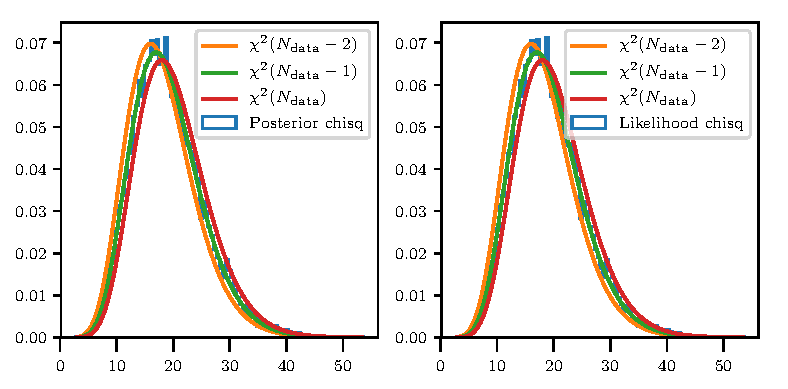
\includegraphics[scale=0.9]{Prior_driven.pdf}
\caption{Prior driven case: In this case, the first way of computing degrees of
freedom reproduces the $\chisq_{\rm lik}$ and the second way of computing
degrees of freedom reproduces $\chisq_{\rm post}$. The cosmic shear analysis is
closer to this case rather than the first.}
\label{fig2}
\end{figure*}

\end{document}
